\documentclass[submission,copyright,creativecommons]{eptcs}
\providecommand{\event}{ICLP 2024} % Name of the event you are submitting to

\usepackage{iftex}

\ifpdf
  \usepackage{underscore}         % Only needed if you use pdflatex.
  \usepackage[T1]{fontenc}        % Recommended with pdflatex
\else
  \usepackage{breakurl}           % Not needed if you use pdflatex only.
\fi

\usepackage[utf8]{inputenc}
\usepackage[english]{babel}
\usepackage{url}
\usepackage{amssymb}
\usepackage{amsmath}
\usepackage{graphicx}
\usepackage{amsthm}

\def\method{\text MixMin~}
\def\methodnospace{\text MixMin}
\def\genmethod{$\mathbb{R}$\text Min~}
\def\genmethodnospace{ $\mathbb{R}$\text Min}

% Highlighting for your Maude, Real-Time Maude, Maude files.
% 
% Source: http://www.github.com/garyyread
% Author: Gary Read
% Contact: garyyread@gmail.com
%
% Using this HI-Maude, Real-Time Maude, Maude listing:
% \lstinputlisting[language = maude]{SOURCE.maude}
%
% or
%
% \begin{lstlisting}[language=maude]
% ***
% *** Maude Source Code
% ***
% \end{lstlisting}

\usepackage{listings}
\usepackage{xcolor}

\definecolor{delimiterColor}{HTML}{B65E47}
\definecolor{numberColor}{HTML}{FF0000}
\definecolor{commentColor}{HTML}{008000}
\definecolor{keyColor}{HTML}{002BFF}

\lstdefinelanguage{maude}
{
	%numbers=left,
	breaklines=true,
	extendedchars=true,
	tabsize=2,
	%frame=shadowbox,
	columns=fullflexible,
	showtabs=false,
	showstringspaces=false,
	showspaces=false,
	showstringspaces=false,
	identifierstyle={\ttfamily},
	keywordstyle={\color{keyColor}},
	ndkeywordstyle={\color{keyColor}},
	stringstyle={\color{delimiterColor}},
	commentstyle={\color{commentColor}},
	ndkeywords={},
	keywords={pr, protecting, sort, sorts, op, ops, var, vars,eq, cq, ceq, crl, rl, mb, cmb, endfm, fmod, is, mod, endm, =, ==, =/=, ctor, ditto, Object, owise, Oid, prec, assoc, id, if, class, homod, endhom, eof, var, vars, eq, op, ops, pr, inc, protecting, including, ceq, is, tomod, endtom, sort, subsort, subsorts, to, endom, fmod, endfm, mod, endm, endtm, comm, gather, fth, endfth, format, metadata, memo},
	morecomment={[l]{***}},
	morecomment={[l]{---}},
}
%\usepackage[toc,page]{appendix}

\renewcommand\UrlFont{\color{blue}\rmfamily}

%\theoremstyle{definition}
\newtheorem{definition}{Definition}[section]

\newtheorem{lemma}{Lemma}[section]

\newtheorem{property}{Property}[section]


\begin{document}


%% The "title" command
\title{Modular Stochastic Rewritable Petri Nets}

\author{Lorenzo Capra
\institute{
	{Dipartimento di Informatica}\\ {Universit{\`a} degli Studi di Milano}, Italy
}
}

\def\titlerunning{Modular Stochastic Rewritable Petri Nets}
\def\authorrunning{Lorenzo Capra}

\maketitle

\begin{abstract}  
Test time scaling is currently one of the most active research areas that shows promise after training time scaling has reached its limits.
Deep-thinking (DT) models are a class of recurrent models that can perform easy-to-hard generalization by assigning more compute to harder test samples.
However, due to their inability to determine the complexity of a test sample, DT models have to use a large amount of computation for both easy and hard test samples.
Excessive test time computation is wasteful and can cause the ``overthinking'' problem where more test time computation leads to worse results.
In this paper, we introduce a test time training method for determining the optimal amount of computation needed for each sample during test time.
We also propose Conv-LiGRU, a novel recurrent architecture for efficient and robust visual reasoning. 
Extensive experiments demonstrate that Conv-LiGRU is more stable than DT, effectively mitigates the ``overthinking'' phenomenon, and achieves superior accuracy.
\end{abstract}  

\section{Introduction}
\label{sec:intro}
\section{Introduction}


\begin{figure}[t]
\centering
\includegraphics[width=0.6\columnwidth]{figures/evaluation_desiderata_V5.pdf}
\vspace{-0.5cm}
\caption{\systemName is a platform for conducting realistic evaluations of code LLMs, collecting human preferences of coding models with real users, real tasks, and in realistic environments, aimed at addressing the limitations of existing evaluations.
}
\label{fig:motivation}
\end{figure}

\begin{figure*}[t]
\centering
\includegraphics[width=\textwidth]{figures/system_design_v2.png}
\caption{We introduce \systemName, a VSCode extension to collect human preferences of code directly in a developer's IDE. \systemName enables developers to use code completions from various models. The system comprises a) the interface in the user's IDE which presents paired completions to users (left), b) a sampling strategy that picks model pairs to reduce latency (right, top), and c) a prompting scheme that allows diverse LLMs to perform code completions with high fidelity.
Users can select between the top completion (green box) using \texttt{tab} or the bottom completion (blue box) using \texttt{shift+tab}.}
\label{fig:overview}
\end{figure*}

As model capabilities improve, large language models (LLMs) are increasingly integrated into user environments and workflows.
For example, software developers code with AI in integrated developer environments (IDEs)~\citep{peng2023impact}, doctors rely on notes generated through ambient listening~\citep{oberst2024science}, and lawyers consider case evidence identified by electronic discovery systems~\citep{yang2024beyond}.
Increasing deployment of models in productivity tools demands evaluation that more closely reflects real-world circumstances~\citep{hutchinson2022evaluation, saxon2024benchmarks, kapoor2024ai}.
While newer benchmarks and live platforms incorporate human feedback to capture real-world usage, they almost exclusively focus on evaluating LLMs in chat conversations~\citep{zheng2023judging,dubois2023alpacafarm,chiang2024chatbot, kirk2024the}.
Model evaluation must move beyond chat-based interactions and into specialized user environments.



 

In this work, we focus on evaluating LLM-based coding assistants. 
Despite the popularity of these tools---millions of developers use Github Copilot~\citep{Copilot}---existing
evaluations of the coding capabilities of new models exhibit multiple limitations (Figure~\ref{fig:motivation}, bottom).
Traditional ML benchmarks evaluate LLM capabilities by measuring how well a model can complete static, interview-style coding tasks~\citep{chen2021evaluating,austin2021program,jain2024livecodebench, white2024livebench} and lack \emph{real users}. 
User studies recruit real users to evaluate the effectiveness of LLMs as coding assistants, but are often limited to simple programming tasks as opposed to \emph{real tasks}~\citep{vaithilingam2022expectation,ross2023programmer, mozannar2024realhumaneval}.
Recent efforts to collect human feedback such as Chatbot Arena~\citep{chiang2024chatbot} are still removed from a \emph{realistic environment}, resulting in users and data that deviate from typical software development processes.
We introduce \systemName to address these limitations (Figure~\ref{fig:motivation}, top), and we describe our three main contributions below.


\textbf{We deploy \systemName in-the-wild to collect human preferences on code.} 
\systemName is a Visual Studio Code extension, collecting preferences directly in a developer's IDE within their actual workflow (Figure~\ref{fig:overview}).
\systemName provides developers with code completions, akin to the type of support provided by Github Copilot~\citep{Copilot}. 
Over the past 3 months, \systemName has served over~\completions suggestions from 10 state-of-the-art LLMs, 
gathering \sampleCount~votes from \userCount~users.
To collect user preferences,
\systemName presents a novel interface that shows users paired code completions from two different LLMs, which are determined based on a sampling strategy that aims to 
mitigate latency while preserving coverage across model comparisons.
Additionally, we devise a prompting scheme that allows a diverse set of models to perform code completions with high fidelity.
See Section~\ref{sec:system} and Section~\ref{sec:deployment} for details about system design and deployment respectively.



\textbf{We construct a leaderboard of user preferences and find notable differences from existing static benchmarks and human preference leaderboards.}
In general, we observe that smaller models seem to overperform in static benchmarks compared to our leaderboard, while performance among larger models is mixed (Section~\ref{sec:leaderboard_calculation}).
We attribute these differences to the fact that \systemName is exposed to users and tasks that differ drastically from code evaluations in the past. 
Our data spans 103 programming languages and 24 natural languages as well as a variety of real-world applications and code structures, while static benchmarks tend to focus on a specific programming and natural language and task (e.g. coding competition problems).
Additionally, while all of \systemName interactions contain code contexts and the majority involve infilling tasks, a much smaller fraction of Chatbot Arena's coding tasks contain code context, with infilling tasks appearing even more rarely. 
We analyze our data in depth in Section~\ref{subsec:comparison}.



\textbf{We derive new insights into user preferences of code by analyzing \systemName's diverse and distinct data distribution.}
We compare user preferences across different stratifications of input data (e.g., common versus rare languages) and observe which affect observed preferences most (Section~\ref{sec:analysis}).
For example, while user preferences stay relatively consistent across various programming languages, they differ drastically between different task categories (e.g. frontend/backend versus algorithm design).
We also observe variations in user preference due to different features related to code structure 
(e.g., context length and completion patterns).
We open-source \systemName and release a curated subset of code contexts.
Altogether, our results highlight the necessity of model evaluation in realistic and domain-specific settings.






\section{(Stochastic) PT nets, \texttt{Maude}, and demonstrative example}
\label{sec:backgr}
\section{Background}\label{sec:backgrnd}

\subsection{Cold Start Latency and Mitigation Techniques}

Traditional FaaS platforms mitigate cold starts through snapshotting, lightweight virtualization, and warm-state management. Snapshot-based methods like \textbf{REAP} and \textbf{Catalyzer} reduce initialization time by preloading or restoring container states but require significant memory and I/O resources, limiting scalability~\cite{dong_catalyzer_2020, ustiugov_benchmarking_2021}. Lightweight virtualization solutions, such as \textbf{Firecracker} microVMs, achieve fast startup times with strong isolation but depend on robust infrastructure, making them less adaptable to fluctuating workloads~\cite{agache_firecracker_2020}. Warm-state management techniques like \textbf{Faa\$T}~\cite{romero_faa_2021} and \textbf{Kraken}~\cite{vivek_kraken_2021} keep frequently invoked containers ready, balancing readiness and cost efficiency under predictable workloads but incurring overhead when demand is erratic~\cite{romero_faa_2021, vivek_kraken_2021}. While these methods perform well in resource-rich cloud environments, their resource intensity challenges applicability in edge settings.

\subsubsection{Edge FaaS Perspective}

In edge environments, cold start mitigation emphasizes lightweight designs, resource sharing, and hybrid task distribution. Lightweight execution environments like unikernels~\cite{edward_sock_2018} and \textbf{Firecracker}~\cite{agache_firecracker_2020}, as used by \textbf{TinyFaaS}~\cite{pfandzelter_tinyfaas_2020}, minimize resource usage and initialization delays but require careful orchestration to avoid resource contention. Function co-location, demonstrated by \textbf{Photons}~\cite{v_dukic_photons_2020}, reduces redundant initializations by sharing runtime resources among related functions, though this complicates isolation in multi-tenant setups~\cite{v_dukic_photons_2020}. Hybrid offloading frameworks like \textbf{GeoFaaS}~\cite{malekabbasi_geofaas_2024} balance edge-cloud workloads by offloading latency-tolerant tasks to the cloud and reserving edge resources for real-time operations, requiring reliable connectivity and efficient task management. These edge-specific strategies address cold starts effectively but introduce challenges in scalability and orchestration.

\subsection{Predictive Scaling and Caching Techniques}

Efficient resource allocation is vital for maintaining low latency and high availability in serverless platforms. Predictive scaling and caching techniques dynamically provision resources and reduce cold start latency by leveraging workload prediction and state retention.
Traditional FaaS platforms use predictive scaling and caching to optimize resources, employing techniques (OFC, FaasCache) to reduce cold starts. However, these methods rely on centralized orchestration and workload predictability, limiting their effectiveness in dynamic, resource-constrained edge environments.



\subsubsection{Edge FaaS Perspective}

Edge FaaS platforms adapt predictive scaling and caching techniques to constrain resources and heterogeneous environments. \textbf{EDGE-Cache}~\cite{kim_delay-aware_2022} uses traffic profiling to selectively retain high-priority functions, reducing memory overhead while maintaining readiness for frequent requests. Hybrid frameworks like \textbf{GeoFaaS}~\cite{malekabbasi_geofaas_2024} implement distributed caching to balance resources between edge and cloud nodes, enabling low-latency processing for critical tasks while offloading less critical workloads. Machine learning methods, such as clustering-based workload predictors~\cite{gao_machine_2020} and GRU-based models~\cite{guo_applying_2018}, enhance resource provisioning in edge systems by efficiently forecasting workload spikes. These innovations effectively address cold start challenges in edge environments, though their dependency on accurate predictions and robust orchestration poses scalability challenges.

\subsection{Decentralized Orchestration, Function Placement, and Scheduling}

Efficient orchestration in serverless platforms involves workload distribution, resource optimization, and performance assurance. While traditional FaaS platforms rely on centralized control, edge environments require decentralized and adaptive strategies to address unique challenges such as resource constraints and heterogeneous hardware.



\subsubsection{Edge FaaS Perspective}

Edge FaaS platforms adopt decentralized and adaptive orchestration frameworks to meet the demands of resource-constrained environments. Systems like \textbf{Wukong} distribute scheduling across edge nodes, enhancing data locality and scalability while reducing network latency. Lightweight frameworks such as \textbf{OpenWhisk Lite}~\cite{kravchenko_kpavelopenwhisk-light_2024} optimize resource allocation by decentralizing scheduling policies, minimizing cold starts and latency in edge setups~\cite{benjamin_wukong_2020}. Hybrid solutions like \textbf{OpenFaaS}~\cite{noauthor_openfaasfaas_2024} and \textbf{EdgeMatrix}~\cite{shen_edgematrix_2023} combine edge-cloud orchestration to balance resource utilization, retaining latency-sensitive functions at the edge while offloading non-critical workloads to the cloud. While these approaches improve flexibility, they face challenges in maintaining coordination and ensuring consistent performance across distributed nodes.



\paragraph{Running example: fault-tolerant production line}
\label{sec:exe}
% !TEX root = main.tex

\begin{figure}[t]
\vspace{-1.5cm}
\begin{minipage}{0.34\textwidth}
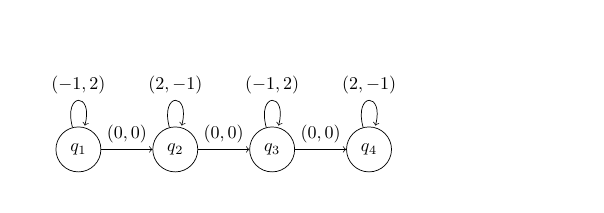
\begin{tikzpicture}[scale=0.25]
\usetikzlibrary{automata, positioning}
\scalebox{0.65}{
\node[state] (q1) {$q_1$};
\node[state, right=of q1] (q2) {$q_2$};
\node[state, right=of q2] (q3) {$q_3$};
\node[state, right=of q3] (q4) {$q_4$};

\path[->] (q1) edge [loop above] node[above] {$(-1,2)$} (q1) edge node[above] {$(0,0)$} (q2); 
\path[->] (q2) edge [loop above] node[above] {$(2,-1)$} (q2) edge node[above] {$(0,0)$} (q3);
\path[->] (q3) edge [loop above] node[above] {$(-1,2)$} (q3) edge node[above] {$(0,0)$} (q4);
\path[->] (q4) edge [loop above] node[above] {$(2,-1)$} (q4);
}
\end{tikzpicture}
\end{minipage}
\begin{minipage}{0.32\textwidth}
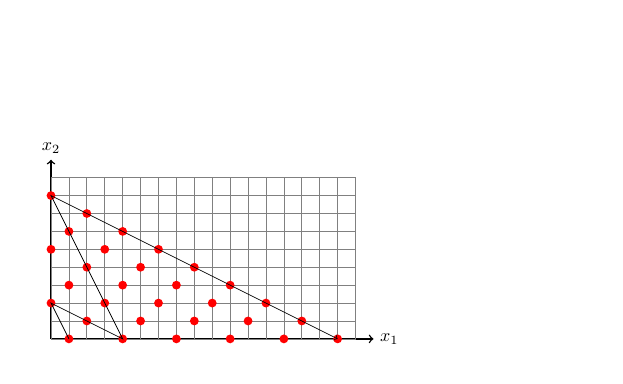
\begin{tikzpicture}[scale=0.35]
\scalebox{0.65}{
\draw[->, thick] (0, 0) -- (18, 0) node[right] {$x_1$};
\draw[->, thick] (0, 0) -- (0, 10) node[above] {$x_2$};

\draw[step=1, gray, thin] (0, 0) grid (17, 9);

\foreach \x in {1,4,7,10,13,16} \fill[red] (\x,0) circle (7pt);
\foreach \x in {2,5,8,11,14} \fill[red] (\x,1) circle (7pt);
\foreach \x in {0,3,6,9,12} \fill[red] (\x,2) circle (7pt);
\foreach \x in {1,4,7,10} \fill[red] (\x,3) circle (7pt);
\foreach \x in {2,5,8} \fill[red] (\x,4) circle (7pt);
\foreach \x in {0,3,6} \fill[red] (\x,5) circle (7pt);
\foreach \x in {1,4} \fill[red] (\x,6) circle (7pt);
\foreach \x in {2} \fill[red] (\x,7) circle (7pt);
\foreach \x in {0} \fill[red] (\x,8) circle (7pt);

\draw[->] (1,0) -- (0,2) -- (2,1) -- (4,0) -- (3,2) -- (2,4) -- (1,6) -- (0,8) -- (2,7) -- (4,6) -- (6,5) -- (8,4) -- (10,3) -- (12,2) -- (14,1) -- (16,0);
}
\end{tikzpicture}
\end{minipage}
\begin{minipage}{0.32\textwidth}
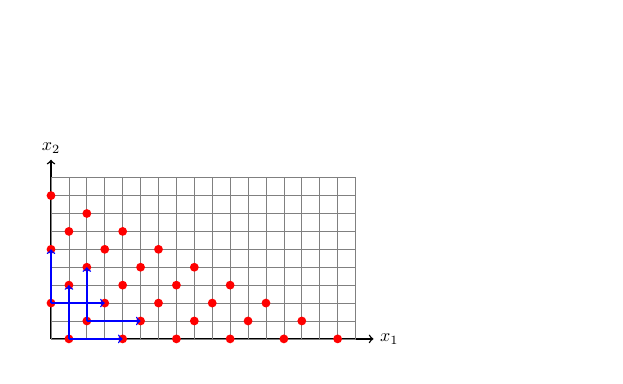
\begin{tikzpicture}[scale=0.35]
\scalebox{0.65}{
\draw[->, thick] (0, 0) -- (18, 0) node[right] {$x_1$};
\draw[->, thick] (0, 0) -- (0, 10) node[above] {$x_2$};

\draw[step=1, gray, thin] (0, 0) grid (17, 9);

\foreach \x in {1,4,7,10,13,16} \fill[red] (\x,0) circle (7pt);
\foreach \x in {2,5,8,11,14} \fill[red] (\x,1) circle (7pt);
\foreach \x in {0,3,6,9,12} \fill[red] (\x,2) circle (7pt);
\foreach \x in {1,4,7,10} \fill[red] (\x,3) circle (7pt);
\foreach \x in {2,5,8} \fill[red] (\x,4) circle (7pt);
\foreach \x in {0,3,6} \fill[red] (\x,5) circle (7pt);
\foreach \x in {1,4} \fill[red] (\x,6) circle (7pt);
\foreach \x in {2} \fill[red] (\x,7) circle (7pt);
\foreach \x in {0} \fill[red] (\x,8) circle (7pt);

\draw[->,blue,thick] (1,0) -- (4,0);
\draw[->,blue,thick] (1,0) -- (1,3);

\draw[->,blue,thick] (2,1) -- (5,1);
\draw[->,blue,thick] (2,1) -- (2,4);

\draw[->,blue,thick] (0,2) -- (3,2);
\draw[->,blue,thick] (0,2) -- (0,5);
}
\end{tikzpicture}
\end{minipage}
\caption{Left: 4-component \dvass $V_2$. 
Middle: the set $\reach_{q_4}(V_2, q_1(1,0))$ and a path $q_1(1,0) \tran q_4(16,0)$.
Right: bases 
%$A = \{(1,0),(2,1),(0,2)\}$ 
and periods 
%$P = \{(0,3),(3,0)\}$
 of an over-approximating semi-linear set $A+P^*$.}
\label{fig:zigzag}
\end{figure}

\begin{example}
For $k\geq 1$, let $V_k$ be a $(2k)$-component \dvass, where each component has just one state $q_i$
and one transition:
$(q_i, (-1,2), q_i)$ for odd $i$, and $(q_i, (2,-1), q_i)$ for even $i$.
Bridge transitions are $(q_i, (0,0), q_{i+1})$.
Figure~\ref{fig:zigzag} shows $V_2$ (left) and 
a path in $V_2$ from $s = q_1(1,0)$ to $t = q_4(16,0)$ together with 
the reachability set $\reach_{q_4}(V_2, s)$ (middle).
In general,
\begin{align} \label{eq:reachk}
X_k := \reach_{q_{2k}}(V_k, s) \ = \ \set{(x_1,x_2) \mid x_1+2x_2 \leq 4^k, \  x_1+2x_2 \equiv 1 \!\! \mod 3}.
\end{align}
Even if the size of the reachability set is 
exponential in $k$, for small $(x_1, x_2)$ it is periodic and the periods are small.
The set $X_k$ can be over-approximated by $A + P^*$ for $A = \set{(1,0),(2,1),(0,2)}$ and $P = \set{(0,3),(3,0)}$
(shown on the right of Figure~\ref{fig:zigzag}), namely for every $k\geq 1$ and $B\in\N$,
the set $X_k$ is \kanapka {$8$} {$B$}. 
For illustration, consider $Y := X_k \cap ((1,0) + P^*)$.
If $(1,0) + P^{\leq B} \subseteq X_k$ then $Y$ is a $B$-approximation
of $(1,0) + P^*$ with $\norm((1,0)), \norm(P) \leq 3 \leq 8$. 
Otherwise, there is some $(v_1, v_2) \in \big((1,0) + P^{\leq B}\big)\setminus X_k$, and
then $B$ is larger than $4^k$:
\[
%8B \geq 2(1 + 3B) \geq 2(v_1 + v_2) \geq v_1 + 2 v_2 > 
4^k < v_1 + 2 v_2 \leq 2(v_1 + v_2) \leq 2(1+3B) \leq 8B.
\]
Therefore by \eqref{eq:reachk}, each $(x_1,x_2) \in Y$ satisfies 
$\norm(x_1,x_2) = x_1 + x_2 \leq x_1 + 2x_2 \leq 4^k < 8B$, and thus
$Y$, seen as a union of singletons, is a union of 
linear sets with norm of base bounded by $8B$ and empty set of periods. 
In both cases, 
$Y$ is \kanapka {$8$} {$B$}. 
%The same intuition stays behind polynomial approximability of \dvass stated in Lemma~\ref{lem:2vass-sandwich}.
\end{example}


\section{Modular Rewritable Stochastic PN: Symmetries and Lumpability}
\label{sec:rewPT}
Rewritable stochastic PT nets (RwSPT) build upon the concept of \emph{modular} rewritable PT nets \cite{CAPRA-TCS2024} by linking negative exponential rates to the firing of PT transitions and the process of net rewrites.
%priorities and stochastic parameters. An RwSPT serves as an algebraic model of a Generalized Stochastic PN \cite{GSPN1993}, combining rewrite rules with the PT firing mechanism. We here concentrate on stochastic PN consisting of zero-priority transitions, accompanied by an 

The definition of RwSPT includes a hierarchy of \textbf{Maude} modules (e.g., \texttt{BAG}, \texttt{PT-NET}, \texttt{PT-SYSTEM}) described in  \cite{CAPRA-TCS2024}.
The \texttt{Maude} sources can be found in \url{https://github.com/lgcapra/rewpt/tree/main/modSPT}.
RwSPT uses structured annotations to underline the symmetry of the model. It features a concise place-based encoding to aid in state canonization and is based on the functional module \verb|BAG{X}|, which introduces multisets as a complex data type. The commutative and associative \verb|_+_| operator provides an intuitive way to describe a multiset as a weighted sum, for instance, \verb|3 . a + 1 . b|. The sort \verb|Pbag| contains multisets of places.
Each place label (a term of sort \verb|Plab|) is a nonempty list of pairs built of \verb|String| and a \verb|Nat|. Places are uniquely identified by their labels. These pairs represent a symmetric component within a nested hierarchy. Compositional operators annotate places incrementally from right to left: The label suffix represents the root of a hierarchy. 
For example, the 'assembly' place of line 1 in Production Line 2 would be encoded as:
%\begin{center}
\verb|p(< "a"; 0 > < "L"; 1 >)|.     
%\end{center}
We implicitly describe net transitions (terms \verb |Tran|) through their incidence matrix (a 3-tuple of terms \verb|Pbag|) and associated tags. A tag includes a descriptive \verb|String|
%, a \verb|Nat| (indicating a priority) 
and a \verb |Float| interpreted as a firing rate. 
%or a probabilistic weight, depending on whether the priority is zero or greater).
The syntax is:
\verb|[I,O,H] -> << S, R >>|. 

Using the associative composition operator \verb"_;_" and the subsort relation \verb"Tran < Net", we can easily construct PT nets in a modular way. For example, we can depict the subnet containing the load transition ($ld$) and a robot ($ln_0$ ) as the \verb"Net" term in the listing below.
%(the zero-arity operator \verb"nilP" represents an empty multi-set).
%in Appendix \ref{apx:ap1}.


{\small\begin{lstlisting}[frame=single,language=maude]
  [2 . p(< "s" ; 0 >), 1 . p(< "w" ; 0 >) + 1 . p(< "w" ; 1 >), nilP] |->  << "ld", 0.5 >> ;
  [1 . p(< "w" ; 0 >), 1 . p(< "a" ; 0 >), 1 . p(< "f" ; 0 > ] |-> << "ln", 0.1 >>
\end{lstlisting}}

A \verb|System| term is the empty juxtaposition (\verb|__|) of a \verb|Net| and a \verb|Pbag| representing the marking. 
The conditional rewrite rule \verb|firing| specifies the PT firing rule
%\footnote{
(notice the use of a matching equation :=).
%: The free variables T, N',
%are matched (:=) against the canonical ground term bound to the variable N.}, as shown in the listing \ref{lst:l2}.
%in Appendix \ref{apx:ap1}.

{\small\begin{lstlisting}[frame=single,language=maude]
 vars N N' : Net . vars T  : Tran . var M : Pbag .
 crl [firing] : N M => N firing(T, M) if T ; N' := N  /\ enabled(T, N M) . 
\end{lstlisting}}

%The predicate \verb|enabled| takes into account priority and 
%relies on \verb|hasConcession|, which determines 
%the 'topological' part of enabling.
%(listing \ref{lst:l2-bis}):

An RwSPT is defined by a system module that contains two constant operators, used as aliases:
\verb|op net : -> Net | and \verb|op m0 : -> Pbag |.
Two equations define their bindings.
This module includes a set $R$ of \verb|System| rewrite rules incorporating \verb|firing|.
We adopt interleaving semantics: Rewrites 
%take the same priority and 
have an exponential rate (specified in the rule label but for \verb|firing|), so that for the state transition system it holds ($\subseteq$ is the subgraph relation):
$TS($\verb|net m0|, $\{$\verb|firing|$\}) \subseteq TS($\verb|net m0|, $R)$.

%Transitioning between the \texttt{Maude} encoding of PT systems and the PNML format adopted by many PN tools is straightforward and reversible.
\vspace{-11pt}
\paragraph{Modularity, symmetries, and lumpability} We have provided net-algebra and net-rewriting operators \cite{CAPRA-TCS2024} with a twofold intention: to ease the modeler's task and to enable the construction and modification of large-scale models with nested components by implicitly highlighting their symmetry.
A compact \emph{quotient} TS is built using simple manipulation of node labels.
This approach outperforms that integrated into \texttt{Maude} \cite{Capra:RP22} and based on traditional graph canonization.

In this context, the identification of behavioral equivalences is reduced to a graph \emph{morphism}. PT system morphism must maintain the edges and the marking: In our encoding,
a \emph{morphism} between PT systems \verb|(N m)| and \verb|(N' m')| is a bijection $\phi \ :$ \verb|places(N)| $\rightarrow$ \verb|places(N')| such that, considering the homomorphic extension of $\phi$ on multisets, $\phi($\verb|N|$) = \ $\verb|N'| and $\phi($\verb|m|$) = \ $\verb|m'|.
Moreover, $\phi$ must retain the textual annotations of the place labels and the transition tags. If \verb|N'| = \verb|N| we speak of \emph{automorphism}, in which case $\phi$ is a permutation in the set of places.
We refer to a \emph{normal} form that principally involves identifying sets of automorphic (permutable) places:
Two markings \verb|m|, \verb|m'| of a net \verb|N| are said automorphic if there is an automorphism $\phi$ in \verb|N| that maps \verb|m| into \verb|m'|.
We denote this \verb|m| $\cong$ \verb|m'|. The equivalence relation $\cong$ is a congruence, that is, it preserves the transition firings and \emph{rates}.
%The next definition helps us simplify the process.
\begin{definition}[Symmetric Labeling]
\label{def:modsym}
A \verb|Net| term is symmetrically labeled if any two maximal sets of places whose labels have the same suffix (possibly empty), which is preceded by pairs with the same tag, are permutable. A \verb|System| term is  symmetrically labeled if its \verb|Net| subterm is.
\end{definition}

\noindent In other words, if a \verb|Net| term \verb|N| meets definition \ref{def:modsym}, then for any two maximal subsets of places matching:

$P := \{$\verb|p(L' < w ; i > L)|$\}, \quad P' := \{$\verb|p(L'' < w ; j > L)|$\}$,

where: \verb|L, L', L'' : Plab, w: String, i, j : Nat| 

\noindent there is an automorphism $\phi$ such that $\phi(P) = P'$, $\phi(P') = P$,
%is a  that maps one set to the other,
which is extended as an identity to the rest\footnote{According to the definition of PT morphism, the prefixes \texttt{L'} and \texttt{L''} are consistent in the textual component.}.

If a \verb|System| term adheres to the previous definition, it can be transformed into a 'normal' form by merely swapping indices on the place labels (e.g., i $\leftrightarrow$ j), while still complying with definition \ref{def:modsym}. This normal form is the most minimal according to a lexicographic order within the automorphism class ($\cong$) implicitly defined by \ref{def:modsym}. In contrast to general graph canonization, there is no need for any pruning strategy or backtracking: A monotone procedure is used where the sequence of index swaps does not matter (see \cite{CAPRA-TCS2024}). Efficiency is achieved as the normalized form of the subterm \verb | Net | is derived through basic ``name abstraction``, where at each hierarchical level the indices of structured place labels continuously span from $0$ to $k \in \Nat$.  

The strategy involves providing a concise set of operators that preserve nets' symmetric labelling. This set includes \emph{compositional} operators %(influenced by process algebra)
and operators for \emph{manipulating} nets.
%, such as adding/removing components.
Rewrite rules require these operators to manipulate \verb|System| terms defined in a modular manner. 
Furthermore, rules must adhere to parametricity conditions that limit the use of ground terms \cite{CAPRA-TCS2024}.
%\paragraph{Lumpability}
Under these assumptions, we get a \emph{quotient} TS from a \verb|System|
term that
retains reachability and
meets strong bisimulation. 

Let $t,t',u,u'$ be (final) terms of sort \verb|System|, 
%$\hat{t}$ the normal form of $t$,
$r$ a \verb|System| rule $r : \ s \Rightarrow s'$. The notation $t \overset{r(\sigma)}{\Rightarrow} t'$
%($t$ is rewritten into $t'$ through $r$)
means there is a ground substitution $\sigma$ of $r$'s variables such that $\sigma(s) = t$ and $\sigma(s')= t'$.
%which meets Definitions \ref{def:symr},\ref{prop:symbr}, 
%and $\hat{r} : \ s \Rightarrow normalize(s')$
%(if we refer to terms that meet Definition \ref{def:modsym}, $u \cong t$ is equivalent to $\hat{u} = \hat{t}$).
%If $\sigma$ is a ground substitution of $r$'s variables and $\phi$ is a morphism between $t$ and $t'$ (i.e., a map from the places of $t$ to the places of $t'$), then $\phi(\sigma)$ is the ground assignment induced by $\phi$ (we recall that \verb|Net| and \verb|System| terms are built of \verb|Place| terms). 
\begin{property}
\label{prop:transition-corr}
Let
%rule $r$ meet Definitions~\ref{def:symr},~\ref{prop:symbr} and 
$t$ meet Definition \ref{def:modsym}.
%\begin{itemize}
    %\item[-] If $t \overset{r(\sigma)}{\Rightarrow} t'$ then $ \exists  \sigma' : \hat{t} \overset{\hat{r}(\sigma')}{\Rightarrow} \hat{t}'$ ($t'$ meets Definition \ref{def:modsym})
    %, where $\phi$ is a morphism $t \rightarrow \hat{t}$.
%\item[-] If $\hat{t} \overset{\hat{r}(\sigma)}{\Rightarrow} \hat{t}'$ then $\forall u \cong t$ $\exists \sigma', u' \cong t' : \ u \overset{r(\sigma')}{\Rightarrow} u'$ ($u'$ meets Definition \ref{def:modsym})
%where $\phi$ is a morphism $t  \rightarrow  u$.
If $t \overset{r(\sigma)}{\Rightarrow} t'$, then $\forall u, \phi, t \cong_{\phi} u$: $ u \overset{r(\phi(\sigma))}{\Rightarrow} u'$, $ t' \cong u'$ 
%($u', t'$ meet the definition \ref{def:modsym})
%\end{itemize}
\end{property}

The TS quotient generated by a normal form $\hat{t}$ is obtained by applying the operator \verb|normalize| to the terms on the right side of the rewrite rules. When a \verb|System| undergoes a rewrite due to the \verb|firing| rule, the process only involves the marking subterm.
%This means applying \verb|normalize| (which is overloaded) to the 
%right-hand side of rule 
%subterm \verb | firing (T, M)| 
%in the listing 1.2.
According to property \ref{prop:transition-corr} (firing preservation), because the morphism $\phi$ preserves the transition rates and the rules are parameterized, it is feasible to map the TS quotient of $\hat{t}$ onto an isomorphic "lumped" CTMC: In a Markov process's state space, an equivalence relation is considered "strong lumpability" if the cumulative transition rates between any two states within a class to any other class remain consistent. Despite the possibility of establishing a more stringent condition, namely "exact lumpabability," we focus on the aggregated probability.
%if the cumulative transition rates from states of an equivalence class into each state of another (or the same class) are all equal.


%\noindent \textbf{Example}
%To demonstrate the aforementioned concepts, we will outline a model of a modular Production System with graceful degradation (Section \ref{sec:exe}). Initially, it is composed of $N$ Production Lines (PL) that share raw materials, with each PL split into $K$ interchangeable lines.
%We first define the net transitions and then build a PL using the \verb"repl&share" operator. The term \verb"PL(K)" represents a line with \verb"K" symmetric branches (Figure 1, top). The structure of the submodel is expressed by adding a pair with the tag \verb|"L"| to the place labels. For example, \verb|p(< "w" ; 0 > < "L" ; 1 >)| describes the "working" place of line 1 of the Production Line. We can choose to exclude places to share among replicas: In this case, we exclude those representing the "warehouse" (tag "s") and faults (tag "o"). Additionally, we can indicate transitions to share: For instance, "load" and "assembly" are shared.
%As a result, the incident input/output edges are weight-\verb|K|.

%The term \verb | Net | \verb | NPL(N, K)| consists of \verb|N| PLs, each of which contains \verb|K| branches. This net was generated using the \verb|repl&share| operator, which adds the \verb|"PL"| tag to place labels to indicate an additional nesting level. The sharing mechanism ensures each PL gathers \verb|K| raw pieces. The PT net represented by \verb|NPL(2,2)| can be seen in Figure \ref{fig:symPL-degarde2}, top-right. Furthermore, the term \verb | System | \verb | NPLsys (N, K, M) | is a PT system that holds \verb|K*M| tokens in the 'warehouse' place, with a single token in each place tagged with \verb|"o"| to trigger fault occurrences within a PL.
%We can build an identical model using the "symmetric" version of the process algebra ALT operator.
%The \verb|System| term generated using the above operators possesses symmetrical labeling (refer to definition \ref{def:modsym}), and its \verb|Net| subterm has already been normalized. 
%Consider, e.g., \verb|NPLsys(2, 2, 1)|.
%By triggering the conflicting transitions "load", which are initially enabled, the following two markings (essentially, subterms of the \verb|System| terms) can be obtained:

%\begin{itemize}
%\item[$m_1$] \verb|p(< "o"; 0 > < "PL"; 0 >) + p(< "o"; 0 > < "PL"; 1 >) +|

%\verb|p(< "w"; 0 > < "L"; 0 > < "PL"; 1 >) + p(< "w"; 0 > < "L"; 1 > < "PL"; 1 >)|

%\item[$m_2$] \verb|p(< "o"; 0 > < "PL"; 0 >) + p(< "o"; 0 > < "PL"; 1 >) +| 

%\verb|p(< "w"; 0 > < "L"; 0 > < "PL"; 0 >) + p(< "w"; 0 > < "L"; 1 > < "PL"; 0 >)|.
%\end{itemize}

%These are automorphic (one can be converted into the other by interchanging \verb|< "PL"; 1 >| \(\leftrightarrow\) \verb|< "PL"; 0 >|), but the second marking is the smallest in lexicographic order and hence corresponds to the normalized form.

%A rewrite rule encapsulates the self-adjustment of a PL with $K=2$ in response to a fault, allowing it to function at diminished capacity (Figure \ref{fig:symPL-degarde2}).
%This rule deviates slightly from \cite{CAPRA-TCS2024}, as it is locally activated by a breakdown, leading to a significantly larger TS. Skipping technical details, we point out that the rule meets the parameterity and only employs operators that uphold the definition \ref{def:modsym}, such as \verb | join |, \verb | detach |, \verb | setMark |. 
%A similar rule removes a faulty and degraded PL from the system. These rules are based on net-operators that retain symmetrical labeling (definition \ref{def:modsym}).
%With the model-checking facilities of \texttt{Maude} (command \texttt{search}), it is possible to formally demonstrate that for any given $N$, the quotient transition system has two absorbing states: Every state comprises a deteriorated PL that contains all $2 \cdot M$ parts (unprocessed, except possibly one).
%This is equivalent to the command below, which yields the same results as its unconditioned counterpart.
%\begin{verbatim}
%search NPLsys(N,2,M) =>! F:System such that 
%net(F:System) == faultyPL /\ B:Pbag := marking(F:System) /\ 
%| match(B:Pbag, "w") | + | match(B:Pbag, "a") | == %2 * M  .    
%\end{verbatim}


%%ARRIVATO QUI
 

\section{Getting the Lumped CTMC generator from RwSPT}
\label{sec:CTMC}
A rewritable PT \texttt{system}  generates a transition system (TS) isomorphic to a lumped CTMC. 
However, the TS produced via the \texttt{show search graph} command of \texttt{Maude} embodies a \emph{parametric} CTMC: in line with the rewriting logic semantics, state transitions denote \emph{classes} of equivalent rewrites, meaning, PT firings that result in identical normalized markings or net rewrites that lead to isomorphic PT systems.

%Consider, e.g., the marking $m_2$ of the previous example: %which matches a normalized form. 
%We can easily verify that this marking enables two equivalent transitions "line" ($ln_i$) and two equivalent transitions "fault" ($ft_i$), respectively, that lead to equivalent (automorphic) markings.
To obtain the CTMC generator, it is necessary to quantify instances that align with a specific state transition. Regrettably, the \texttt{Maude} system lacks a mechanism to determine the matches of a rewrite rule in the TS construction process.

%To achieve our goal,
%We have three possible strategies.
%\begin{enumerate}
%    \item Use a partial "edge unfolding" operator to calculate all possible rewrites from a normalized source state to a normalized target state of the TS. It requires post-processing the TS generated by \texttt{Maude}.
%    \item Use \texttt{Maude}'s meta-level to establish meta-rules that can identify potential matches of base rules.
%    \item 
  Our solution consists of first (automatically) generating a Transition System with states having a composite structure, which provides a detailed view of the equivalent rewrites that result in state transitions. Subsequently, using elementary parse to compute the cumulative rates of the lumped CTMC.
%\end{enumerate}
 %The second strategy, although elegant, has been shown far from efficient. Because efficiency is our primary concern, we have opted for a middle-ground solution: the third strategy.
 Despite a redundant state representation, this method incurs an acceptable time overhead because it only involves \emph{normalized} states. 
 %It relies on two operators. The first operator provides potential matches for each rule considering the subset of independent variables involved, and then the second emulates the rewriting process. It is possible to automatically define these two operators from the syntax of a rule. 
 %To better illustrate the idea, refer to the listing \ref{lst:l5} in Appendix \ref{apx:ap1}.

%The state structure defined by the mixfix constructor \verb|StateTranSys| comprises four fields. The initial pair describes the PT system, while the remaining two fields detail the state transitions caused by the \verb|firing| rule and other rewrites, in that order. We collect state transitions that share the target for calculating aggregated rates. Let us take the \verb|firing| rule as an example: it has two associated operators, namely \verb|enabled|, which gives the set of possible transitions, and \verb|fire|, which provides the reached markings,
%(in their normal form),
%each one prefixed by a multiset of transition tags. We proceed analogously for other rules.

%The operator \verb|toStateTran| converts the conventional state representation into a structured one. The firing rule is adapted easily.
When considering the term \verb|NPLsys(2,2,2)|, which aligns with the PT net at the top left of Figure \ref{fig:symPL-degarde2}, the resulting quotient TS comprises 295 states compared to the 779 states in the standard TS. State transitions often correspond to multiple matches: For instance, the initial state (the term above) includes two 'load' instances and four 'fault' instances that lead to markings with identical normal forms. Consequently, the combined rates are $2\cdot0.5$ and $4\cdot0.001$. 
%Equivalent rewrites of the net structure are observed when $N > 2$. 

\vspace{-10pt}
\paragraph{Experimental Evidence}
We showcase experimental validation of the method and a demonstration of standard performance indicators. Table \ref{tab:perf} displays the results of the \texttt{search} command to locate the final states.
We used Linux WSL on an 11th Gen. Intel Core i5 with 40GB RAM. The state spaces match those of the lumped CTMC. The analysis of large models is feasible solely by exploiting the model's symmetry.
Notice that the number of absorbing states in the TS quotient does not vary with $N$. 
%In \cite{CAPRA-TCS2024}, the effectiveness of modular RwPT was compared to that of Symmetric Nets (SN, previously known as well-formed nets) \cite{CHIOLA97}, a colored Petri net that generates a symbolic reachability graph equivalent %(in its stochastic extension)
%to a lumped CTMC. A parametric SN model was developed, whose unfolding coincides with \verb| NPLsys (N, K, M)|
%but without the degradation process.
%As the values of N and K increase, the degree of state aggregation in modular RwPT significantly exceeds that of SN. For instance, when N=10, K=3, and M=3, the degree of state aggregation is about 45 times that of SN, and when N=10, K=4, and M=3, it is about 200 times that of SN.

%\vspace{-3pt}
%As an example of performance metrics, 
Figure
%\ref{fig:PlotX} shows the system throughput, while 
\ref{fig:PlotRel} shows the system \emph{reliability} (the complement of Time to System Failure distribution).
%as a time function. 
As expected, %both 
is decreases with time; additionally, the scenario that involves more replicas demonstrates
%increased throughput and
enhanced reliability.
The inflexion point at around time 800
%in both curves
represents the system's reconfiguration time. The increased execution time of the job (not reported) is a result of a system failure.
The overall trend is also noticeable when we look at larger values of \verb|N|. As \verb|N| increases, both reliability and throughput curves show significant improvements.
However, we observe an asymptotic trend when \verb|N| is greater than 6. Our interpretation is that beyond a certain point, the benefit of using a higher number of replicas is outweighed by the higher fault rate and the increased configuration overhead.

\vspace{-0.5cm}
\begin{table}[htbp]
\centering\small
\caption{Ordinary vs Quotient TS of \texttt{NPLsys(N,2,2)} \hspace{2pt} ${}^\dag$ \texttt{search} timed out after 10 h} 
\label{tab:perf}
\begin{tabular}{ |p{0.5cm}||p{2.5cm}p{1.5cm}||p{2.5cm}p{1.5cm}| }
\hline
 & \multicolumn{2}{c||}{Ordinary} & \multicolumn{2}{|c|}{Quotient} \\
\verb|N|   & states(final)  & time (sec) &  states(final) & time (sec) \\
\hline
\hline
1   &    60(2) & 0 &      42(2) & 0\\
\hline
2   &    779(4) & 0.1 &     295(2) & 0.1\\
\hline
3  &   6101(6) & 4.8  &  1059(2) & 0.9\\
\hline
4 &    37934(8) & 69 & 2764(2) & 3.6\\
\hline
5 &   204362(10) & 818 & 5970(2) & 10 \\
\hline
6 &   1000187(12) & 13930 & 11367(2) & 27\\
\hline
7 &  - & ${}^\dag$ & 19775(2) & 65 \\
\hline
8 &  - & ${}^\dag$ &  32144(2) & 186 \\
\hline
9 & - & ${}^\dag$ &  49554(2) & 569 \\
\hline
10 & - & ${}^\dag$ & 73215(2) & 2450 \\ 
\hline
\end{tabular}
\end{table}
%\begin{figure}[htbp]
%   \begin{center}    
%    \includegraphics[clip,trim={2.1cm 2.7cm 2.2cm 2.2cm},width=0.85\columnwidth]{figures/PlotThroughput.pdf}
%    \end{center}
%    \caption{System Throughput.}
%    \label{fig:PlotX}
%\end{figure}

\begin{figure}[htbp]
   \begin{center}    
    \includegraphics[clip,trim={2.1cm 2.7cm 2.2cm 2.2cm},width=0.7\columnwidth]{figures/PlotReliability.pdf}
    \end{center}
    \caption{System Reliability.}
    \label{fig:PlotRel}
\end{figure}

%To evaluate the system's performance, Figure \ref{fig:PlotXdivRel} shows the throughput while the system is operational, which is the ratio between the graphs in Figures \ref{fig:PlotX} and \ref{fig:PlotRel}. It can be seen that the throughput approaches that of a single line, which, given the parameters, is $1/202.5 = 4.98E-03$.

%\begin{figure}[htbp]
%   \begin{center}    
%    \includegraphics[clip,trim={2.1cm 2.7cm 2.2cm 2.2cm},width=0.85\columnwidth]{figures/PlotConditionedThroughput.pdf}
%    \end{center}
%    \caption{System Throughput conditioned to its reliability.}
%    \label{fig:PlotXdivRel}
%\end{figure}



\section{Conclusion and Future Work}
We have developed a lumped Markov process for modular and rewritable Petri nets (RwPT), a flexible model of adaptive distributed systems.
%encoded in \texttt{Maude}.
RwPTs, which we construct and manipulate using a small set of algebraic operators, exhibit structural symmetries that result in an efficient quotient state-transition graph.
%Using an example of a gracefully degrading system,
We have outlined a semi-automatic procedure for deriving the CTMC infinitesimal generator from the RwPT quotient graph. Future efforts will focus, on the one hand, on exploring orthogonal structured solutions and, on the other, on fully implementing the process and integrating it into graphical editors.
%such as \texttt{DrawNET} (\url{https://www.draw-net.com/}). 
%Simultaneously,
We aim to broaden the approach
%on one side,
to derive a lumped Markov process 
%from rewritable GSPN, and on the other, to extract the infinitesimal CTMC generator
from any \texttt{Maude} specification.


%% Define the bibliography file to be used
\bibliographystyle{eptcs}
\bibliography{lc}

\end{document}
\newpage
\appendix
\section{Appendix: Figures and \texttt{Maude} excerpts}
\label{apx:ap1}

\begin{figure}[htbp]
   \begin{center}    
    \begin{tabular}{c}
        \fbox{\includegraphics[scale=0.5]{figures/PL}}\\
        $\Downarrow$\\

  \fbox{\includegraphics[scale=0.5]{figures/degrPL}}
    \end{tabular}
    \end{center}
    \caption{Production Line (PL) and adaptation following a fault.}
    \label{fig:FMS}
%\end{figure}

%\begin{figure}[htbp]
   \begin{center}    
    \begin{tabular}{rl}
        \fbox{\includegraphics[scale=0.33]{figures/2PL}}&
        $\Rightarrow$
        \fbox{\includegraphics[scale=0.33]{figures/2PL1F}}
        $\Rightarrow$\\
        $~$&$~$\\
        $\Rightarrow$
        \fbox{\includegraphics[scale=0.33]{figures/2PL2F}}&
        $\Rightarrow$
        \fbox{\includegraphics[scale=0.33]{figures/2PLfinal}}
    \end{tabular}
    \end{center}
    \caption{One of the possible paths of the Gracefully Degrading Production System.}
    \label{fig:symPL-degarde2}
\end{figure}

\noindent The following are the listings relevant to the procedures described in this paper.

{\small
\begin{lstlisting}[frame=single,caption=Topological enabling condition \label{lst:l2-bis},language=maude]
vars X Y Z X' : Pbag .
op hasConcession : Tmatrix  Pbag -> Bool .
eq hasConcession([X,Y,Z], X') = X <= X' and-then Z > X' .
\end{lstlisting}}

{\small
\begin{lstlisting}[frame=single,,caption=Modular Specification of a Fault Tolerant Production System \label{lst:l3},language=maude]
fmod FTPL is
 pr NET-OP{SPTlab} .
 ops PL PLA nomPL faultyPL NfaultyPL : NzNat -> Net . 
 op faultySys : NzNat -> System . 
 op NPL  : NzNat NzNat -> Net [memo]. 
 op NPLsys : NzNat NzNat NzNat -> System . 
 ops loadLab asLab failLab workLab : -> Tlab [memo] .
 eq loadLab = << "ld",0, 0.5 >> .
 eq asLab = << "as",0, 2.0 >> .
 eq workLab = << "ln",0, 0.1 >> .
 eq failLab = << "ft",0, 0.001 >> .
 var I  : Nat . 
 vars N K M : NzNat .
 eq line =  [1 . p(< "w" ; 0 >),1 . p(< "a" ; 0 >),1 . p(< "f" ; 0 >) ] |-> workLab .
 eq fault = [1 . p(< "o" ; 0 >) , 1 . p(< "f" ; 0 >), nilP ] |-> failLab .
 eq load  = [1 . p(< "s" ; 0 >) , 1 . p(< "w" ; 0 >) , nilP ] |-> loadLab .
 eq ass   = [1 . p(< "a" ; 0 >) , 1 . p(< "s" ; 0 >)  , nilP ]  |-> asLab .
 eq cycle = load ; line ; ass ; fault .
 eq PL(K) = repl&share(cycle, K, "L", p (< "o" ; 0 >) U p(< "s" ; 0 >), asLab U loadLab) .
 eq NPL(N, K) = repl&share(PL(K), N, "PL", p(< "s" ; 0 >), emptyStlab) . 
 eq NPLsys(N, K, M) = setMark(setMark(NPL(N, K), "o" "PL", 1), "s", K * M) .
 ...
endfm
\end{lstlisting}
}

{\small
\begin{lstlisting}[frame=single,caption=Rewrite rule of a PL (the label contains the rule's exponential rate) \label{lst:l4},language=maude,label=list:rewrules]
vars S S' S'' : Pbag .
vars I  J : Nat .
var Sys Sys' : System .
var L : Lab .
crl [r1-0.005] : N  S => normalize(join(Sys, setMark(setMark(Sys', "w" "fPL", | match(S', "w") |), "a" "fPL", | match(S', "a") |)))  
if  S'' + 1 . p(< "f" ; J > L < "PL" ; I >) := S /\ N' := nomPL(I) /\ dead (N' S) /\ S' := subag(S'', < "PL" ; I >) /\ Sys := detache(N, N') S'' - S' /\ Sys' := faultySys(notIn(N, "fPL"))  .
\end{lstlisting}
}

{\small
\begin{lstlisting}[frame=single,caption=TS encoding for the lumped CTMC \label{lst:l5} ,language=maude,label=list:rewrules]
var N : Net .
vars M M' : Pbag .  
var  TS    : TagSet .
var  FS   : Fset .
var  RS   : Rset .
op NET:_ M:_ FIRING:_REW:_ : Net Pbag Fset Rset -> StateTranSys [ctor] .
op toStateTran : System -> StateTranSys . 
eq toStateTran(N M) = NET: N  M: M FIRING: fire(enabled(N M), M) REW: allRew(N M) . 
***
rl [sfiring] : NET: N M: M FIRING: (TS --> M', FS) REW: RS => toStateTran(N M') .

\end{lstlisting}
}


%%
%% If your work has an appendix, this is the place to put it.
%\appendix

%\section{Appendix - Maude specification of rewritable PT nets}
%\section{Proofs from Section~\ref{sec:gammaok}} \label{app:gamma}

\subsection{On the girth of locally \texorpdfstring{$\gamma$}{gamma}-sparse graphs}
\begin{lemma}\label{lemma:girth_rev}
    Let $G = (V,E)$ be an undirected graph with girth $g(G)$.
    Then $G$ is \ok{0} if and only if $g(G) \geq 5$.
\end{lemma}
\begin{proof}
    We first prove that if $G$ is \ok{0} then $g(G)$ must be at least $5$.
    In order to prove that, we simply negate the statement and prove that if $G$ has girth $<5$ then $G$ can not be \ok{0}.
    Without loss of generality, assume that $g(G) = 4$ (the case $g(G) = 3$ is similar).
    Then there must exist a cycle $C = (u_1, u_2, u_3, u_4)$ of $4$ vertices.
    It is simple to see that $u_2,u_4 \in \lset_1(u_1)$ and $u_3 \in \lset_2(u_1)$.
    Since $u_3$ is a neighbor of both $u_2$ and $u_4$, the degree of $u_3$ in the subgraph $G\left[\lset_1(u_1) \cup \{u_4\} \right]$ is at least $2$, hence $G$ is not \ok{0} (see \Cref{subfig:girth1}).
    
    We now prove that if $g(G) \geq 5$ then $G$ must be \ok{0}.
    Again, we negate this statement and prove that if $G$ is not \ok{0} then the girth of $G$ must be less then $5$.
    Let us assume that $G$ is \gammaok, for any $\gamma > 0$, thus it is not \ok{0}.
    Since $G$ is not \ok{0} there exists a vertex $v \in V$ such that at least one of the following properties holds (see \Cref{subfig:girth2}):
    \begin{enumerate}
        \item $\exists u \in \lset_1(v)$ such that the degree of $u$ in $G\left[ \lset_1(v) \right]$ is greater then $0$, or;
        \item $\exists w \in \lset_2(v)$ such that the degree of $w$ in $G\left[ \lset_1(v) \cup \{ w \} \right]$ is greater then $1$.
    \end{enumerate}
    In the first case, we have a cycle of $3$ vertices, then $g(G) = 3$.
    In the second case, we have a cycle of $4$ vertices, then $g(G) = 4$.
    In both cases $g(G) < 5$.
\end{proof}
\begin{figure}[h]
    \centering
    \begin{subfigure}[b]{0.35\linewidth}
            \centering
            \includegraphics[width=\linewidth]{img/girth-1.pdf}
            \caption{}
            \label{subfig:girth1}
    \end{subfigure}
    \begin{subfigure}[b]{0.6\linewidth}
            \centering
            \includegraphics[width=\linewidth]{img/girth-2.pdf}
            \caption{}
            \label{subfig:girth2}
    \end{subfigure}%
    \caption{}
    \label{fig:example_girth}
\end{figure}

\subsection{Deterministic lazy-update on \texorpdfstring{$\gamma$}{gamma}-sparse graphs}\label{apx:gamma-ok-deterministic}

\begin{theorem}\label{lemma:gamma-ok-error-bound-balls}
    
Let $\varepsilon \in (0,1)$, and let $G^{(0)}$ be an initial graph. Consider any sequence of edge insertions that yields a final graph $G$. If $G$ is \gammaok, \lazyscheme$(\varphi = \frac{\varepsilon}{1 - \varepsilon},k=0)$ has an approximation ratio of  $\frac{\gamma + 1}{1-\varepsilon}$ and amortized update cost $O(1/\varepsilon)$. 
    
\end{theorem}
\begin{proof}
Recall that $\bd_u$ denotes the black degree of $u$, and that  \Cref{alg:det_thresh} guarantees that $\deg_u$ is at most $(1+\varphi)\bd_u$.
    Then, it is simple to give an upper bound to the size of $\ball_2(u)$, that is $\vert \ball_2(u) \vert \leq 1+ \sum_{v \in \lset_1(u)} (1 + \varphi)\bd_v$.Consider a vertex $v \in \lset_1(u)$. Since $G$ is \gammaok, the number of neighbors of $v$ belonging to $\lset_2(u)$ is at lest $\deg_v - (\gamma+1)$ of which $\bd_v - (\gamma+1)$ must belong to $\apxball_2(u)$. Moreover, a vertex in $\lset_2(u)$ has at most $\gamma+1$ neighbors in $\lset_1(u)$. Therefore: 
    \begin{align*}
    \vert \apxball_2(u) \vert
    &\geq  \bd_u + 1 + \frac{1}{\gamma + 1}\sum_{v \in \lset_1(u)}(\bd_v - (\gamma + 1))\\
    &= \bd_u + 1 + \frac{1}{\gamma + 1}\sum_{v \in \lset_1(u)}\bd_v - \underbrace{\frac{1}{\gamma + 1}\sum_{v \in \lset_1(u)}(\gamma + 1)}_{= \bd_u}\\
    &= 1+ \frac{1}{\gamma + 1}\sum_{v \in \lset_1(u)}\bd_v.
    \end{align*}
  
    As a consequence, $\vert \apxball_2(u) \vert/\vert \ball_2(u) \vert \ge \frac{1}{(1+\varphi)(\gamma+1)}$. By setting $\varphi = \frac{\varepsilon}{1 - \varepsilon}$, and by using \Cref{lm:amortized_det_alg},  the claim follows.
\end{proof}

\subsection{Proof of \Cref{le:gamma_ok_expect_lowerbound}}\label{apx:proof_gamma_ok_expect_lowerbound}
\begin{proof}
Let $e_1, \dots, e_{\ell_v}$ be the \emph{red edges} between $v$ and $\lset_2(u)$, and define the binary random variable $\lrdr_v(i)$ that is equal to $1$ if $e_i$ is a \emph{quasi-black edge} for $u$, $0$ otherwise, for $i = 1, \dots, \lrd_v$. Thus we can express $\lrdr_v = \sum_{i=1}^{\lrd_v} \lrdr_v(i)$, with expectation

\begin{equation}\label{eq:gamma_ok_lb_fact_eq_1}
\begin{aligned}
  \Expec{}{\lrdr_v} & = \sum_{i=1}^{\lrd_v}{\Prob{}{\lrdr_v(i)=1}} = \lrd_v - \sum_{i=1}^{\lrd_v} {\Prob{}{\lrdr_v(i)=0}}.
\end{aligned}
\end{equation}

Without loss of generality, assume that the edges $e_1, \dots, e_{\lrd_v}$ have been inserted at times $t_1 < \dots < t_{\lrd_v}$, respectively.
If $e_i$ is not a quasi-black edge for $u$, then it must be that $u$ is not selected by $v$ at \Cref{line:random_selection} of \Cref{alg:det_thresh}, at times $t_i, t_{i+1},\dots, t_{\lrd_v}$.
This holds with probability 
\begin{equation}\label{eq:gamma_ok_lb_fact_eq_2}
\begin{aligned} 
    &\Prob{}{\lrdr_v(i) = 0}
    \leq \prod_{j=i}^{\lrd_v} \left( 1-\frac{k}{\deg_v^{(t_j)}} \right)
    \leq \prod_{j=i}^{\lrd_v} \left( 1 - \frac{k}{\deg_{v}^{(t_{\lrd_v})}} \right) \\
    &\leq \left( 1-\frac{k}{\lbdd_v + \lrd_v + \gamma + 1}\right)^{\lrd_v - i + 1} 
    \leq \left(1-\frac{k}{2(\lbdd_v + \gamma + 1)}\right)^{\lrd_v - i}.
\end{aligned}
\end{equation}
The third inequality holds since the edges incident to $v$ having endpoints in $L_1(u)$ are at most $\gamma$, while those having endpoints in $L_2(u)$ are exactly $\lbdd_v+ \lrd_v$. Moreover, the last inequality holds because $\lrd_v \leq \rd_v \leq \bd_v \leq \lbdd_v + \gamma + 1$, given the assumption $\varphi = 1$.

By plugging in \eqref{eq:gamma_ok_lb_fact_eq_2} into   \eqref{eq:gamma_ok_lb_fact_eq_1} and we obtain
\begin{align*}
    &\Expec{}{\lrdr_v} \geq \lrd_v - \sum_{i=1}^{\lrd_v}\left( 1-\frac{k}{2(\lbdd_v + \gamma + 1)}\right)^{\lrd_v - i} \\
    &= \lrd_v - \sum_{i=0}^{\lrd_v-1} \left(1-\frac{k}{2(\lbdd_v + \gamma + 1)}\right)^i 
    \leq \lrd_v - \frac{1-\left(1-\frac{k}{2(\lbdd_v+\gamma+1)}\right)^{\lrd_v}}{1-\left(1-\frac{k}{2(\lbdd_v + \gamma + 1)}\right)} \\
    &\geq \lrd_v - \frac{1}{1-\left(1-\frac{k}{2(\lbdd_v + \gamma + 1)}\right)}
    \geq \lrd_v - \frac{2(\lbdd_v + \gamma + 1)}{k}.
\end{align*}
\end{proof}

%\section{Appendix - auxiliary Maude modules}
%\section{Declarations}
%=======================================================================
%
\subsection{Acknowledgements}
%
Hagen Holthusen and Tim Brepols gratefully acknowledge financial support of the projects 417002380 and 453596084 by the Deutsche Forschungsgemeinschaft.
In addition, Kevin Linka is supported by the Emmy Noether Grant 533187597 by the Deutsche Forschungsgemeinschaft.
This work was supported by the NSF CMMI Award 2320933 Automated Model Discovery for Soft Matter and by the ERC Advanced Grant 101141626 DISCOVER to Ellen Kuhl.
%
%=======================================================================
%
\subsection{Conflict of interest}
%
The authors of this work certify that they have no affiliations with or involvement in any organization or entity with any financial interest (such as honoraria; participation in speakers’ bureaus; membership, employment, consultancies, stock ownership, or other equity interest; and expert testimony or patent-licensing arrangements), or non-financial interest (such as personal or professional relationships, affiliations, knowledge or beliefs) in the subject matter or materials discussed in this manuscript.
%=======================================================================
%
\subsection{Availability of data and material}
%
Our data used for training and testing are accessible to the public at \url{https://doi.org/10.5281/zenodo.14894687}
%=======================================================================
%
\subsection{Code availability}
%
Our source code and examples of the iCANN implementation in JAX are accessible to the public at \url{https://doi.org/10.5281/zenodo.14894687}.
%=======================================================================
%
\subsection{Contributions by the authors}
%
\textbf{Hagen Holthusen:} Conceptualization, Methodology, Software, Validation, Formal analysis, Investigation, Data Curation, Writing - Original Draft, Writing - Review \& Editing, Visualization, Funding acquisition\\
\textbf{Kevin Linka:} Methodology, Writing - Original Draft, Writing - Review \& Editing, Funding acquisition\\
\textbf{Ellen Kuhl:} Methodology, Writing – Original draft, Writing – review \& editing, Funding acquisition\\
\textbf{Tim Brepols:} Methodology, Writing - Original Draft, Writing - Review \& Editing, Funding acquisition\\
%=======================================================================
%
\subsection{Statement of AI-assisted tools usage}
%
This document was prepared with the assistance of OpenAI's ChatGPT, an AI language model. ChatGPT was used for language refinement. The authors reviewed, edited, and take full responsibility for the content and conclusions of this work.
